% simdoc.tex V3.0, 30 March 2010

\documentclass[times]{simauth}

\usepackage{moreverb}

%\usepackage[T1,mtbold]{mathtime} % commented by ShareLaTeX Team because of compilation errors

\usepackage[
%dvips, % commented by ShareLaTeX Team because of compilation errors
colorlinks,bookmarksopen,bookmarksnumbered,citecolor=red,urlcolor=red]{hyperref}

\usepackage[utf8]{inputenc}
\usepackage[T1]{fontenc}
\usepackage[spanish]{babel}
\usepackage{wrapfig}
\usepackage{framed}
\usepackage{upquote}
\usepackage{epigraph}
\usepackage{makeidx}
\graphicspath{ {images/} }

%\newcommand{\mysmall}{\fontsize{7.5pt}{8pt}\selectfont}

%\newcommand\BibTeX{{\rmfamily B\kern-.05em \textsc{i\kern-.025em b}\kern-.08em
%T\kern-.1667em\lower.7ex\hbox{E}\kern-.125emX}}

\def\volumeyear{2010}

\begin{document}

%\runninghead{A.~N.~Other}

\title{
    {\fontfamily{ppl} \fontsize{30}{1} \selectfont{
        Tarea \#3:\\ Falacias de razonamiento en medios de comunicación nacional}
    }
}

\author{
    {\fontfamily{ppl} \fontsize{14}{1} \selectfont{
        Carlos Martín Flores González \\
        Raquel Rodríguez Chaves}
    }
}

%\address{John Wiley \& Sons, Ltd, The Atrium, Southern Gate, Chichester,
%West Sussex, PO19~8SQ, UK}
%
%\corraddr{Journals Production Department, John Wiley \& Sons, Ltd,
%The Atrium, Southern Gate, Chichester, West Sussex, PO19~8SQ, UK.}

%\begin{abstract}
%This paper describes the use of the \LaTeXe\ \textsf{simauth.cls}
%class file for setting papers for \emph{Statistics in Medicine}.
%\end{abstract}

%\keywords{class file; \LaTeXe; \emph{Statist.\ Med.}}

\maketitle

\tableofcontents

\section{Introducción}

\newpage
\section{Falacia 1: Diputado equipara Costa Rica con la Alemania Nazi}
\begin{table}[h!]
    \begin{tabular}{ll} 
        \toprule[1.5pt]
        Fuente & Periódico \href{http://elmundo.cr}{elmundo.cr}\\
        \midrule[0.5pt]
        Fecha  & 9 de setiembre 2015\\
        \midrule[0.5pt]
        Falacia & Palabras emotivas \\
        \bottomrule[1.5pt]
    \end{tabular} 
\end{table}

El legalización de técnicas de Fertilización in Vitro (FIV) ha resultado ser un tema muy polémico en nuestro país, principalmente en la asamblea legislativa en donde un pequeño grupo de diputados de partidos conservadores se oponen a la utilización de esta técnica aduciendo que atenta contra la vida humana.

En su discurso de la sesión del día martes 8 de setiembre del 2015, el diputado Gonzalo Ramírez Zamora, un claro opositor del FIV, llegó a comparar a Costa Rica con la Alamania Nazi diciendo que: \textit{``Hoy, los grandes campos de exterminio pasaron de la Alemania nazi a la Costa Rica en la que hoy estamos viviendo, los grandes campos de exterminio pasaron de la Alemania nazi a la Costa Rica de la Administración Solís Rivera, eso es una barbaridad, ese es un decreto contra la vida, eso es decreto que no es restrictivo y que deja abierta la posibilidad de que en un laboratorio cualquiera fecunde la cantidad de óvulos que se le antoje, una barbaridad, no existe jurídicamente un derecho a los hijos''}.

En su discurso el diputado Ramírez hace un claro uso de palabras emotivas con el fin de despertar sentimientos negativos ante la posible aprobación de esta técnica, de esta forma tanto diputados presentes, seguidores de su partido y público en general podrían llegar a crear sentimientos de miedo u odio con el fin de generar mayor oposición.


\noindent Dirección: \href{http://www.elmundo.cr/costarica/diputado-equipara-costa-rica-la-alemania-nazi-decreto-la-fiv/}{http://www.elmundo.cr/costarica/diputado-equipara-costa-rica-la-alemania-nazi-decreto-la-fiv/} \\
Discurso del diputado Ramírez: \href{https://www.youtube.com/watch?v=cK6AeaFB1Co}{https://www.youtube.com/watch?v=cK6AeaFB1Co}\\
El detalle de la noticia se puede ver en la figura \ref{fig:falacia1}.

\newpage
\begin{figure}[h]
    \centering
    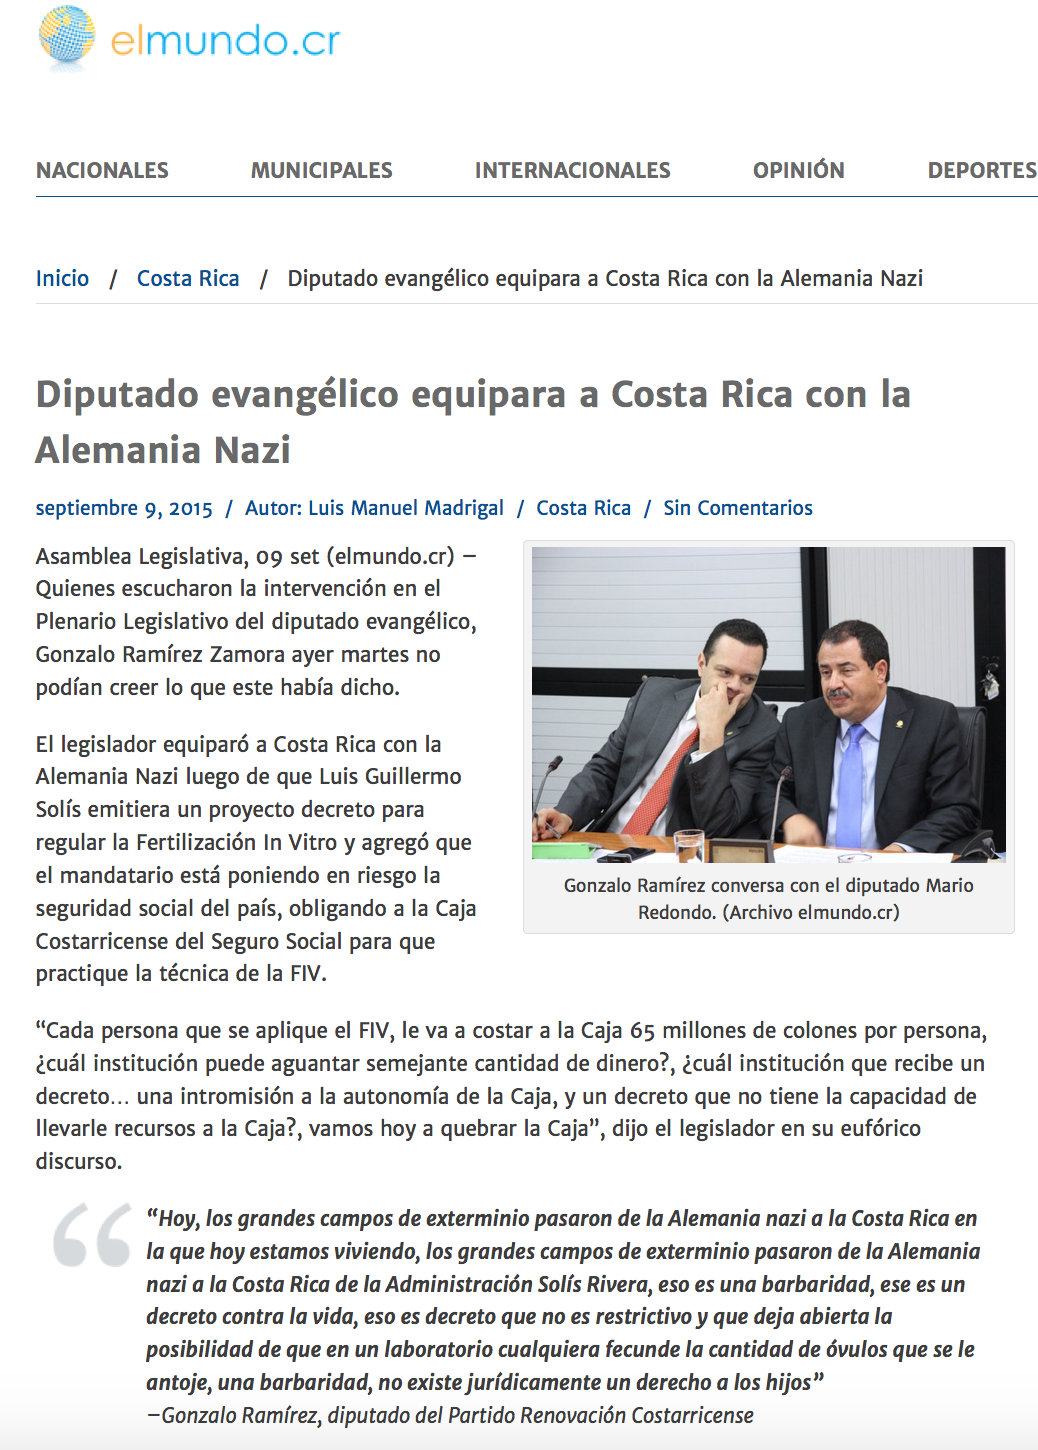
\includegraphics[width=15cm]{costarica-nazi-fiv}
    \captionof{figure}{Captura de pantalla de la noticia}
    \label{fig:falacia1}
\end{figure}


\section{Falacia 2: Lorem Ipsum}

\section{Falacia 3: Lorem Ipsum}

\section{Falacia 4: Lorem Ipsum}

\section{Falacia 5: Lorem Ipsum}

\section{Falacia 6: Lorem Ipsum}

\section{Falacia 7: Lorem Ipsum}

\section{Falacia 8: Lorem Ipsum}

\section{Falacia 9: Lorem Ipsum}

\section{Falacia 10: Lorem Ipsum}

\section{Falacia 11: Lorem Ipsum}

\section{Falacia 12: Lorem Ipsum}


\begin{thebibliography}{9}

\bibitem{R1} Kopka~H, Daly~PW. 2003. \emph{A Guide to \LaTeX} (4th~edn).
Addison-Wesley.

\bibitem{R2} Lamport~L. 1994. \emph{\LaTeX: a Document Preparation System} (2nd~edn).
Addison-Wesley.

\bibitem{R3} Mittelbach~F, Goossens~M. 2004. \emph{The \LaTeX\ Companion}
(2nd~edn). Addison-Wesley.
\end{thebibliography}
\end{document}

